% !TEX root = Technologierecherche.tex
%\subsection{Spurerkennung}
%Damit das Fahrzeug die Strecke autonom abfahren kann, muss das Fahrzeug in der Lage sein, die Spur selbständig zu erkennen.
%Die autonome Spurerkennung kann mit unterschiedlichen mitteln realisiert werden.

\subsection{Erkennung des rechten Randes mit Sensoren}
Der rechte Rand des Parcours ist für die Spurerkennung vielversprechend. Er ist entweder durch eine weisse Linie, ein 5mm hohes Trottoir oder für kurze Zeit auf der Kreuzung nicht begrenzt.
Für die unterschiedlichen Bedingungen werden verschieden Möglichkeiten aufgezeigt.\\

\textbf {Erkennung der weissen Linie} \\
Die rechte Begrenzungslinie ist 1cm breit und weiss. Es gibt viele Minaturfahrzeuge die einer Linie folgen. Jedoch ist bei den meisten Linienfolger die zu folgende Linie in der Mitte des Fahrzeuges. Das hat der Vorteil das man links und rechts der Linie die Linie detektieren kann. Dies ist bei dieser Aufgabenstellung nicht oder nur sehr begrenzt möglich. Dies ist für beide Lösungsvarianten eine Herausforderung. Für beide wäre ein Funktionsmustr nötig.
Hier zwei Möglichkeiten:\\

\begin{figure} [hbp]
	\centering
	\begin{subfigure}[b]{0.4\textwidth}
		\includegraphics[width=\textwidth]{Images/Linienerkennung_1.png}
		\caption{Variante 1. Sensoren über der Linie}
	\end{subfigure}
	\hfill
	\begin{subfigure}[b]{0.42\textwidth}
		\includegraphics[width=\textwidth]{Images/Linienerkennung_2.png}
		\caption{Variante 2. Sensoren neben der Linie}
\end{subfigure}
	\caption{Mögliche Linienerkennungen mit Infrarotsensoren}\label{fig:animals}
\end{figure}

\textbf {Erkennung des Trottoirs}
Das Trottoir ist die längste und wichtigste (rechte) Begrenzung des Tracks. Es ist der längste Strassenabschnitt und die Positionsbestimmung muss a präzisesten funktionieren. Für das die Trottoir Erkennung sind diese zwei Varianten im Vergleich.\\
 
\begin{figure} [hbp]
	\centering
	\begin{subfigure}[b]{0.4\textwidth}
		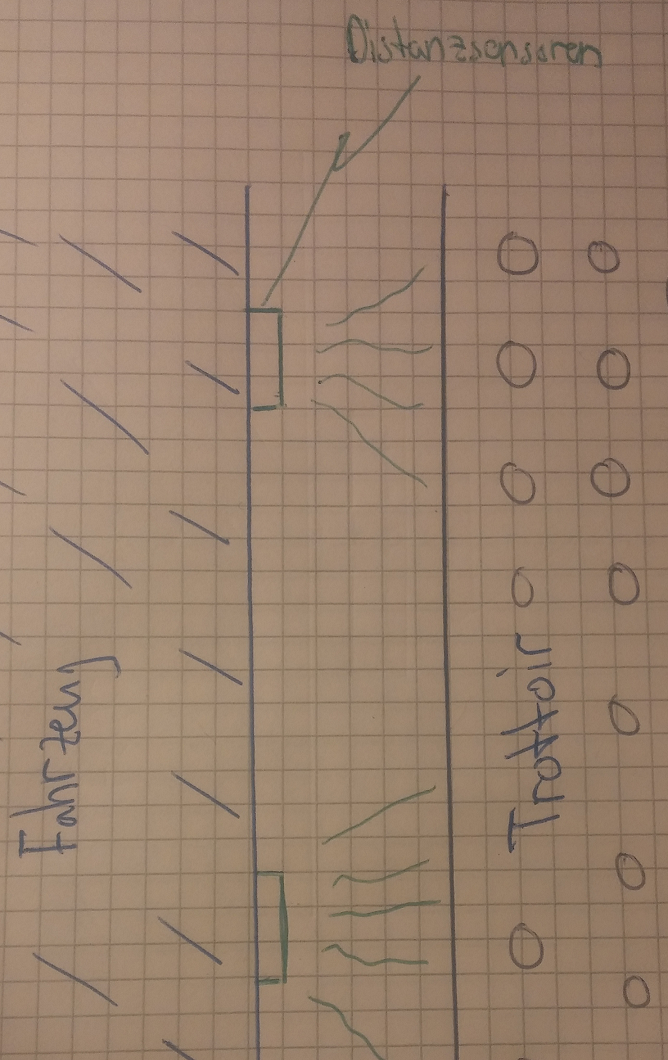
\includegraphics[width=\textwidth]{Images/Trottoirerkennung_1.png}
		\caption{Variante 1. Distanzsensoren als Abstandsmessung}
	\end{subfigure}
	\hfill
	\begin{subfigure}[b]{0.4\textwidth}
		\includegraphics[width=\textwidth]{Images/Trottoirerkennung_2.png}
		\caption{Variante 2. Distanzhalter als mechnische Bregrenzung (z.B Räder)}
\end{subfigure}
	\caption{Mögliche Spurhalte Konzepte beimTrottoir}\label{fig:animals}
\end{figure}

\textbf {Möglichkeiten bei keiner Begrenzung (Kreuzung)} \\
Die Kreuzung ist der Spezialfall des Tracks. Es gibt keine Begrenzung am rechten Rand. 
Da keine Begrenzung vorhanden ist, kann man mit Sensoren auch nicht detektieren.
Die Lösung ohne Sensoren ist bei der Kreuzung stur geradeaus zu fahren. Dies könnte man einprogrammieren, wenn weder eine Linie noch ein Trottior vorhanden ist. Dies setzt natürlich die richtige Ausrichtung des Fahrzeuges vor der Kreuzung voraus.

\subsection{Fest einprogrammierte Strecke ohne Sensoren}
Zu der Variante mit vielen Sensoren gibt es die Möglichkeit die Strecke fest einzuprogrammieren. Da die Strecke immer gleich bleibt (ausser den zwei Möglichen Startplätze) ist es Möglich die Strecke bereits fest einzuprogrammieren.
\textbf {Vorteile}
\begin{itemize}
\item Keine Sensoren für die Spurerkennung notwendig.
\item Kostenersparnis
\item Weniger Fehlerquellen\\
\end{itemize}
\textbf {Nachteile}
\begin{itemize}
\item Keine Fehlerkorrektur (einmal falsch, immer falsch)
\item Braucht extrem genauer Antrieb + Lenkung
\end{itemize}